% !TEX root = ../../../main.tex
% 来源：高中物理甲种本·第一册（力学）
% 章节：曲线运动 / 匀速圆周运动
% 原始文件：4.tex，行 490-508
% 类型：tikz
% ---
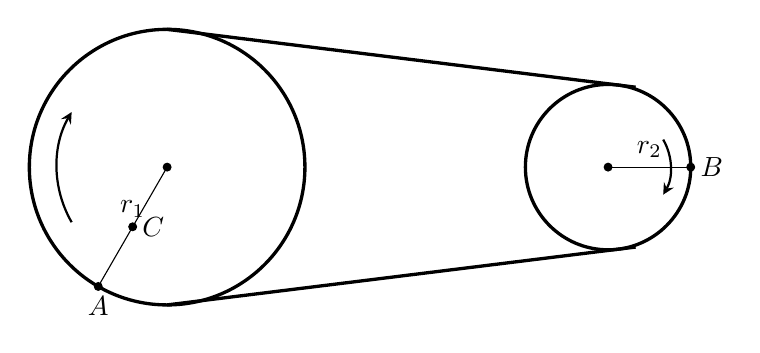
\begin{tikzpicture}[>=stealth, scale=.7]
\draw [very thick](0,0)  circle [radius=2.5];
\draw [very thick](8,0)  circle [radius=1.5];

\draw [->, thick](210:2) arc (210:150:2);
\draw [->, thick](9,.5) arc (30:-30:1);
\draw (0,0)--node [above]{$r_1$}(240:2.5);
\draw (8,0)--node [above]{$r_2$}(9.5,0);

\draw [fill=black] (240:2.5) circle (2pt)node [below]{$A$};
\draw [fill=black] (240:1.25) circle (2pt) node [right]{$C$};
\draw [fill=black] (0,0) circle (2pt) ;
\draw [fill=black] (8,0) circle (2pt) ;
\draw [fill=black] (9.5,0) circle (2pt) node [right]{$B$} ;

\draw [very thick] (0,2.5)--(8.5,1.45);
\draw [very thick] (0,-2.5)--(8.5,-1.45);

\end{tikzpicture}
